\section{A Wait-Free Method for Top-Down BFS}
\label{sec:wf-topdown}

This section presents our BFS method with top-down steps only; Section~\ref{sec:dir-opt} adds bottom-up steps. The method replaces the barrier at the end of each level with bookkeeping that lets every thread decide on its own when a level is complete, and finish any part of it that other threads have left undone. Algorithm~\ref{alg:wf-td} gives the method as thread $t$ runs it.

\subsection{Levels and Buckets}
\label{sec:td-structure}

The levels of a search form a linked list, whose node $N_d$ describes level $d$ (Figure~\ref{fig:td-example}). A node holds its depth $d$, a pointer $\mathit{next}$ to the node of level $d+1$, which is null until some thread links that node, and one \emph{entry} for each thread. Entry $t$ of $N_d$ holds the \emph{bucket} $B_{d,t}$, a list of vertices of level $d$ that thread $t$ has discovered, and two fields that record how far the expansion of the bucket has got: $\mathit{last}_{d,t}$, the position of the last vertex of $B_{d,t}$ that thread $t$ itself has finished, which starts at $-1$, and the flag $\mathit{done}_{d,t}$, which a thread sets once it has finished the vertices of the bucket. Only thread $t$ appends to $B_{d,t}$, and only thread $t$ writes $\mathit{last}_{d,t}$.

Besides the distances, the method keeps a flag $\mathit{vis}[u]$ for every vertex $u$, which marks $u$ as expanded: a thread sets it once it has examined every neighbor of $u$, and other threads then skip $u$. A vertex can be in several buckets of a level, since several threads can discover it at the same time, but every copy is in the right level: a vertex in $B_{d,t}$ is at distance $d$. Before a search, $N_0$ holds the source $s$ in the bucket of thread $0$, $\mathit{dist}[s] = 0$, and every other distance is $-1$ and every flag unset.

\begin{algorithm}
\caption{Wait-free top-down BFS, as thread $t$ runs it. For a node $N = N_d$, $N.B[o]$, $N.\mathit{last}[o]$ and $N.\mathit{done}[o]$ stand for $B_{d,o}$, $\mathit{last}_{d,o}$ and $\mathit{done}_{d,o}$.}
\label{alg:wf-td}
\begin{algorithmic}[1]
\Procedure{BFS}{$s$}
    \State $N \gets N_0$
    \While{$N \neq \mathit{null}$}
        \State \textbf{fence} \label{ln:td-fence}
        \State \Call{ExpandLevel}{$N$}
        \State $N \gets N.\mathit{next}$ \label{ln:td-next}
    \EndWhile
\EndProcedure
\Statex
\Procedure{ExpandLevel}{$N$}
    \For{$k \gets 0$ \textbf{to} $T-1$}
        \State $o \gets (t + k) \bmod T$
        \IfThen{$N.\mathit{done}[o]$ \textbf{or} $N.B[o]$ is empty}{\textbf{continue}}
        \IfThen{$N.\mathit{next} = \mathit{null}$}{\Call{AddLevel}{$N$}} \label{ln:td-add}
        \State $\mathit{size} \gets$ the size of $N.B[o]$ \label{ln:td-size}
        \If{$o = t$}
            \For{$i \gets 0$ \textbf{to} $\mathit{size}-1$} \label{ln:td-own}
                \State \Call{Expand}{$N$, $N.B[t][i]$}
                \State $N.\mathit{last}[t] \gets i$ \label{ln:td-last}
            \EndFor
        \Else
            \State $\mathit{first} \gets N.\mathit{last}[o] + 1$ \label{ln:td-first}
            \ForAll{$i$ from $\mathit{first}$ to $\mathit{size}-1$, in a random order} \label{ln:td-help}
                \State \Call{Expand}{$N$, $N.B[o][i]$}
            \EndFor
        \EndIf
        \State $N.\mathit{done}[o] \gets \mathit{true}$ \label{ln:td-done}
    \EndFor
\EndProcedure
\Statex
\Procedure{Expand}{$N$, $u$}
    \IfThen{$\mathit{vis}[u]$}{\textbf{return}}
    \ForAll{neighbors $v$ of $u$}
        \If{$\mathit{dist}[v] = -1$}
            \State append $v$ to $N.\mathit{next}.B[t]$ \label{ln:td-push}
            \State $\mathit{dist}[v] \gets N.\mathit{depth} + 1$ \label{ln:td-dist}
        \EndIf
    \EndFor
    \State $\mathit{vis}[u] \gets \mathit{true}$ \label{ln:td-vis}
\EndProcedure
\Statex
\Procedure{AddLevel}{$N$}
    \State $M \gets$ the spare node of $t$, or a new node
    \State $M.\mathit{depth} \gets N.\mathit{depth} + 1$
    \If{\Call{CAS}{$N.\mathit{next}$, $\mathit{null}$, $M$}} \label{ln:td-cas}
        \State $t$ has no spare node
    \Else
        \State $M$ becomes the spare node of $t$
    \EndIf
\EndProcedure
\end{algorithmic}
\end{algorithm}

\subsection{Expanding a Level}
\label{sec:td-expand}

A thread expands level $d$ by visiting the $T$ entries of $N_d$, starting with its own and continuing with those of threads $t+1$, $t+2$, and so on, modulo $T$ (\textsc{ExpandLevel}). It skips an entry whose bucket is empty or whose flag $\mathit{done}$ is set. Otherwise, it reads the size of the bucket, expands the vertices before that position, sets $\mathit{done}$, and moves on to the next entry.

In its own bucket, a thread expands the vertices in order, and after each one it publishes its position in $\mathit{last}_{d,t}$ (line~\ref{ln:td-last}). In the bucket of another thread $o$, it expands only the vertices after position $\mathit{last}_{d,o}$, the ones $o$ had not finished when the helper read it, and takes them in a random order (line~\ref{ln:td-help}). Expanding a vertex $u$ does nothing if $\mathit{vis}[u]$ is set (\textsc{Expand}). Otherwise, the thread examines every neighbor $v$ of $u$, and if $\mathit{dist}[v] = -1$, it appends $v$ to its own bucket in $N_{d+1}$ and sets $\mathit{dist}[v] = d+1$. After the last neighbor, it sets $\mathit{vis}[u]$.

A thread thus works on its own bucket first, and helps the others once it is done with it. When no thread is delayed, the threads mostly expand their own buckets, and a thread that finishes early takes over part of the work of those still busy. A thread that is delayed, or has stopped for good, holds no one up: the others expand what is left of its bucket, set its flag $\mathit{done}$, and move on.

When a thread has visited all $T$ entries of $N_d$, every vertex of level $d$ has been expanded, by it or by another thread, so every vertex of level $d+1$ has been discovered and is in some bucket of $N_{d+1}$. The thread then moves on to $N_{d+1}$ without waiting for anyone (line~\ref{ln:td-next}). Before it reads the buckets of the new level, it executes a fence (line~\ref{ln:td-fence}), which makes all of its earlier writes visible to the other threads. On x86, its last appends to $N_{d+1}$ could otherwise still sit in its store buffer, where only it sees them, while other threads read the buckets of $N_{d+1}$ (Section~\ref{sec:pf-tso}); the fence costs one instruction per level. In the method of Section~\ref{sec:dir-opt}, the CAS that claims the plan of a level, which comes before any thread expands the level, does the same job, so that method needs no fence. Slower threads may still be expanding level $d$; Section~\ref{sec:td-order} explains why they cannot harm the levels after it, and Section~\ref{sec:proof} proves it.

\subsection{The Order of Writes}
\label{sec:td-order}

Threads skip work on the strength of what other threads have written. A vertex whose distance is set is not discovered again, a vertex whose flag $\mathit{vis}$ is set is not expanded again, helpers do not expand the vertices up to position $\mathit{last}_{d,o}$ of a bucket, and no thread visits a bucket whose flag $\mathit{done}$ is set. Each of these writes comes after the work it lets others skip, so a thread that stops between any two of its steps leaves no work undone that others would skip:
\begin{itemize}
    \item A thread appends $v$ to its bucket, and only then sets $\mathit{dist}[v]$ (lines~\ref{ln:td-push} and~\ref{ln:td-dist}). If it stops in between, $\mathit{dist}[v]$ is still $-1$, and another thread discovers $v$ again and appends it to its own bucket. In the other order, a thread that stopped after setting $\mathit{dist}[v]$ would leave $v$ discovered but in no bucket, and no thread would ever expand it.
    \item A thread sets $\mathit{vis}[u]$ only after it has examined every neighbor of $u$ (line~\ref{ln:td-vis}). A thread that stops in the middle of expanding $u$ leaves $\mathit{vis}[u]$ unset, so other threads expand $u$ again, from its first neighbor.
    \item A thread publishes $\mathit{last}_{d,t} = i$ only after it has finished the vertex at position $i$ of its bucket, and sets $\mathit{done}$ only after it has finished every vertex it read in the bucket (lines~\ref{ln:td-last} and~\ref{ln:td-done}).
\end{itemize}
Every thread that discovers $v$ writes the same distance, $d+1$, so a plain store suffices for it. Section~\ref{sec:dir-opt} replaces the store with a CAS, so that the direction rule counts the edges of each vertex only once.

A delayed thread can also resume long after the others have moved on. Suppose thread $t$ stopped while expanding a vertex $u$ of level $d$, after it read $\mathit{dist}[v] = -1$ for a neighbor $v$ but before it appended $v$. Before any thread could finish level $d$, some thread finished expanding $u$, and in doing so either appended $v$ itself or found it already discovered, and therefore already appended, by another thread. When thread $t$ resumes, it appends $v$ to $B_{d+1,t}$, which the others may have expanded already, and writes $\mathit{dist}[v] = d+1$ again. Neither write does harm: the distance is the one already there, and the late copy of $v$ is in the right level and duplicates one that the others have expanded or will expand, so a thread that read $B_{d+1,t}$ before the late append missed nothing. Such late appends are why a vertex can have several copies in a level, and why $\mathit{done}$ means that the vertices a thread read in a bucket are finished, rather than every vertex the bucket will ever hold.

\subsection{Buckets}
\label{sec:td-buckets}

A bucket has to let its owner append vertices while any number of other threads read it, without locks, and without ever letting a reader see a position that has not been written or memory that has been freed. The readers are helpers, which can read a bucket while its owner is still appending to it, and because of late appends, an owner can append to a bucket long after other threads have read it and moved on. The number of vertices a bucket will hold is not known in advance, and helpers read a bucket by position, starting after $\mathit{last}$ and taking blocks in a random order. A bucket is therefore a dynamic array, and since only its owner writes it, appends need no CAS.

\begin{algorithm}
\caption{Appending to a bucket $B$, which only its owner does, and reading it, which any thread can do.}
\label{alg:bucket}
\begin{algorithmic}[1]
\Procedure{Append}{$B$, $v$}
    \If{$B.\mathit{size} = B.\mathit{capacity}$}
        \State $c \gets \max(2 \cdot B.\mathit{capacity}, c_0)$
        \State $A \gets$ an array of $c$ vertices from the owner's arena
        \State copy $B.\mathit{array}[0], \ldots, B.\mathit{array}[B.\mathit{size}-1]$ into $A$
        \State $B.\mathit{array} \gets A$ \label{ln:bk-array}
        \State $B.\mathit{capacity} \gets c$
    \EndIf
    \State $B.\mathit{array}[B.\mathit{size}] \gets v$
    \State $B.\mathit{size} \gets B.\mathit{size} + 1$ \label{ln:bk-size}
\EndProcedure
\Statex
\Procedure{Read}{$B$}
    \State $s \gets B.\mathit{size}$
    \State $A \gets B.\mathit{array}$
    \State \Return $A[0], \ldots, A[s-1]$
\EndProcedure
\end{algorithmic}
\end{algorithm}

A bucket has three fields: the pointer $\mathit{array}$ to its current array, the number $\mathit{size}$ of vertices appended so far, and the $\mathit{capacity}$ of the current array, which only the owner reads (Algorithm~\ref{alg:bucket}). When the array is full, the owner allocates one twice as large from its arena, copies the vertices into it, and only then publishes it in $\mathit{array}$ (line~\ref{ln:bk-array}); the first array has a small fixed size $c_0$. To append a vertex, the owner writes it at position $\mathit{size}$ of the array, and only then increases $\mathit{size}$ (line~\ref{ln:bk-size}). A reader reads in the opposite order: $\mathit{size}$ first, then $\mathit{array}$, and then the vertices before position $\mathit{size}$. In Algorithm~\ref{alg:wf-td}, a thread reads the size of a bucket at line~\ref{ln:td-size}, and its array only afterwards.

These two orders keep every read within positions that have been written, even when the read overlaps an append that grows the array. Suppose a reader reads the size $s$. Since the owner publishes an array before any size that needs it, and the reader reads the size before the array, the array the reader then finds is the one that was current when $s$ was published, or a later one. The first holds the first $s$ vertices, which are never moved or overwritten, and every later array holds copies of them, made before it was published. Whichever array the reader finds, its first $s$ positions are written and hold the same vertices. A reader can miss vertices appended after it read the size, but that is of no consequence: by the time a thread reads the buckets of $N_d$, every vertex of level $d$ is in them already, and the appends that come later are late copies (Section~\ref{sec:td-order}).

An array that the owner has replaced cannot be freed during the search, since a reader may still hold its pointer, and a delayed reader may hold it for any length of time. Finding out when no reader holds it any more would take extra work from every reader, so old arrays instead stay in the owner's arena until the search is over, and the arenas are reset as a whole once every call has returned. Since capacities double, the old arrays of a bucket together hold fewer positions than its current array, and a bucket of $k$ vertices that has outgrown its first array takes fewer than $4k$ positions in all. An append takes constant time amortized, and the copy in a growth moves at most $n$ vertices, since a thread appends each vertex at most once in a search (Section~\ref{sec:proof}).

\subsection{Linking Levels and Ending the Search}
\label{sec:td-link}

A thread that finds a bucket of $N_d$ to expand first makes sure that $N_{d+1}$ exists, since the vertices it discovers go there (line~\ref{ln:td-add}). If $N_d.\mathit{next}$ is null, the thread prepares a node for level $d+1$ and tries to link it with a CAS on $N_d.\mathit{next}$ from null (line~\ref{ln:td-cas}). If the CAS fails, another thread has linked a node already, and every thread uses that one. A node that lost the race was never seen by any other thread, so its thread keeps it as a spare and tries it again at the next level, instead of allocating another. Threads tend to reach a level together, and nearly all of them prepare a node for the next one, so without spares most of these nodes would be wasted.

A thread links $N_{d+1}$ before it expands any vertex of level $d$, and sets a flag $\mathit{done}$ only afterwards, so a thread that skips a done bucket still finds $N_{d+1}$ linked. A level without vertices, on the other hand, gets no successor: all of its buckets are empty, so no thread links a node after it, and every thread that visits it finds $\mathit{next}$ null and returns (line~\ref{ln:td-next}). The first such level is level $D+1$, where $D$ is the largest distance from $s$, so every call of the method goes through the nodes of levels $0$ to $D+1$ and returns there.

\subsection{An Example}
\label{sec:td-example}

\begin{figure}
    \centering
    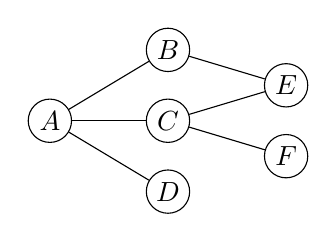
\begin{tikzpicture}[vertex/.style={circle, draw, minimum size=0.55cm, inner sep=0pt}]
        \node[vertex] (A) at (0,0) {$A$};
        \node[vertex] (B) at (1.5,0.9) {$B$};
        \node[vertex] (C) at (1.5,0) {$C$};
        \node[vertex] (D) at (1.5,-0.9) {$D$};
        \node[vertex] (E) at (3,0.45) {$E$};
        \node[vertex] (F) at (3,-0.45) {$F$};
        \draw (A) -- (B);
        \draw (A) -- (C);
        \draw (A) -- (D);
        \draw (B) -- (E);
        \draw (C) -- (E);
        \draw (C) -- (F);
    \end{tikzpicture}

    \vspace{0.3cm}

    \begin{tikzpicture}[>=Stealth, levelnode/.style={draw, rectangle, align=left, font=\footnotesize, minimum width=1.55cm, inner sep=3pt}]
        \node[levelnode] (n0) at (0,0) {$N_0$\\ $0$: $A$\\ $1$: --};
        \node[levelnode] (n1) at (2.05,0) {$N_1$\\ $0$: $B, C$\\ $1$: $C, D$};
        \node[levelnode] (n2) at (4.1,0) {$N_2$\\ $0$: $E$, \textcolor{gray}{$F$}\\ $1$: $F$};
        \node[levelnode] (n3) at (6.15,0) {$N_3$\\ $0$: --\\ $1$: --};
        \draw[->] (n0) -- (n1);
        \draw[->] (n1) -- (n2);
        \draw[->] (n2) -- (n3);
    \end{tikzpicture}
    \caption{A search from $A$ with two threads. Each node lists the buckets of threads $0$ and $1$. Both threads discover $C$, so level 1 holds it twice. Thread $0$ stalls while expanding $C$, and appends $F$ to its bucket in $N_2$ (in gray) only after thread $1$ has finished the search.}
    \Description{A graph with vertices A to F, and the four level nodes of a search from A by two threads, with the buckets of each thread in each node.}
    \label{fig:td-example}
\end{figure}

Figure~\ref{fig:td-example} shows a search from $A$ with two threads. Level 0 holds $A$ in the bucket of thread 0. Thread 1 finds its own bucket empty and helps thread 0, which has not finished $A$ yet, so both threads expand $A$ at the same time. Thread 0 discovers $B$ and $C$, and thread 1, which reads $\mathit{dist}[C]$ just before thread 0 sets it, discovers $C$ and $D$, so level 1 holds $C$ twice. In level 1, thread 0 expands $B$, which discovers $E$, and publishes $\mathit{last}_{1,0} = 0$. It then starts on $C$, reads $\mathit{dist}[F] = -1$, and stalls before it appends $F$. Thread 1 meanwhile expands its own bucket: $C$, which is not marked yet, so thread 1 discovers $F$, and then $D$, which discovers nothing new. It then helps thread 0 with the vertices after position 0 of $B_{1,0}$. The only one is $C$, which thread 1 has just expanded, so it skips it and sets $\mathit{done}_{1,0}$. Thread 1 goes on to expand level 2, which links $N_3$, finds the buckets of $N_3$ empty, and returns. The search is now complete, although thread 0 is still stalled in level 1. When thread 0 resumes, it appends $F$ to $B_{2,0}$, writes $\mathit{dist}[F] = 2$ again, and finishes $C$. It then finds the buckets of $N_2$ done and those of $N_3$ empty, and returns too.

\subsection{Keeping Helpers Apart}
\label{sec:td-contention}

The method is correct whatever order the threads take entries and vertices in; the orders we use keep the threads out of each other's way. Owners walk their buckets in order, which keeps their reads sequential. A helper starts after the owner's published position, and walks the rest of the bucket in small blocks of consecutive entries, taking the blocks in a random order of its own and the vertices of a block in order. Helpers on the same bucket thus rarely expand the same vertex at the same time, or the vertex its owner is on, while each still reads consecutive entries. A vertex with many neighbors raises the same problem within a single expansion: if the owner and helpers expanded it together, walking its neighbors in the same order, they would all write the same entries of $\mathit{dist}$ at the same moment. A helper therefore walks a long neighbor list in small blocks as well, in a random order of its own. Each random order is an affine permutation of the $k$ blocks, which visits block $(a + i b) \bmod k$ in step $i$, for a random $a$ and a random $b$ coprime to $k$, so it takes two random numbers and no memory.
